\documentclass[12pt]{article}
\usepackage[utf8]{inputenc}
\usepackage{upquote}
\usepackage[margin=20mm]{geometry} 
\usepackage{amsmath,amsthm,amssymb}
\usepackage{graphicx}
\usepackage{listings}
\newenvironment{statement}[2][Statement]{\begin{trivlist}
\item[\hskip \labelsep {\bfseries #1}\hskip \labelsep {\bfseries #2.}]}{\end{trivlist}}
\usepackage{xcolor}
\usepackage{subfigure}


% Listings package for code rendering (No external dependencies)
\usepackage{listings}  
\usepackage{xcolor}   % Color support
\usepackage{tcolorbox} % Box for better appearance

% Define custom colors for code highlighting
\definecolor{codegreen}{rgb}{0,0.6,0}
\definecolor{codegray}{rgb}{0.5,0.5,0.5}
\definecolor{codepurple}{rgb}{0.58,0,0.82}
\definecolor{backcolour}{rgb}{0.95,0.95,0.92}


\lstset{frame=tb,
    language=Python,
    backgroundcolor=\color{backcolour},   
    commentstyle=\color{codegreen},
    keywordstyle=\color{magenta},
    numberstyle=\tiny\color{codegray},
    stringstyle=\color{codepurple},
    basicstyle=\ttfamily\footnotesize,
    breakatwhitespace=false,         
    breaklines=true,                 
    keepspaces=true,                 
    numbers=left,       
    numbersep=5pt,                  
    showspaces=false,                
    showstringspaces=false,
    showtabs=false,                  
    tabsize=2,
}




\title{Assignment 2}


%\author{Author \\
%  Wanjing Hu / fng685@alumni.ku.dk  \\
%  Shuangcheng Jia/   \\
%  Zhigao Yan / sxd343@alumni.ku.dk  \\
%} 
 

\begin{document}
\maketitle

\section{Pixel-wise contrast enhancement}
\subsection{Gray scale Image}
%wanjing
\begin{lstlisting}[caption={Gamma-Prime},captionpos=b]
def gamma_transform(image, gamma):
    # Normalize to [0,1]
    image = image.astype(np.float32) / 255.0 
    # Apply gamma correction
    corrected = np.power(image, gamma) 
    # Convert back to [0,255]
    return (corrected * 255).astype(np.uint8) 
\end{lstlisting}

A gamma=1 is equals to the original gray-scale picture, a gamma=0.5 makes dark regions look brighter, and a gamma=2.0 darkens bright regions. See figure~\ref{fig:1.1} and Listing 1.

\begin{figure}[ht]
\centering
    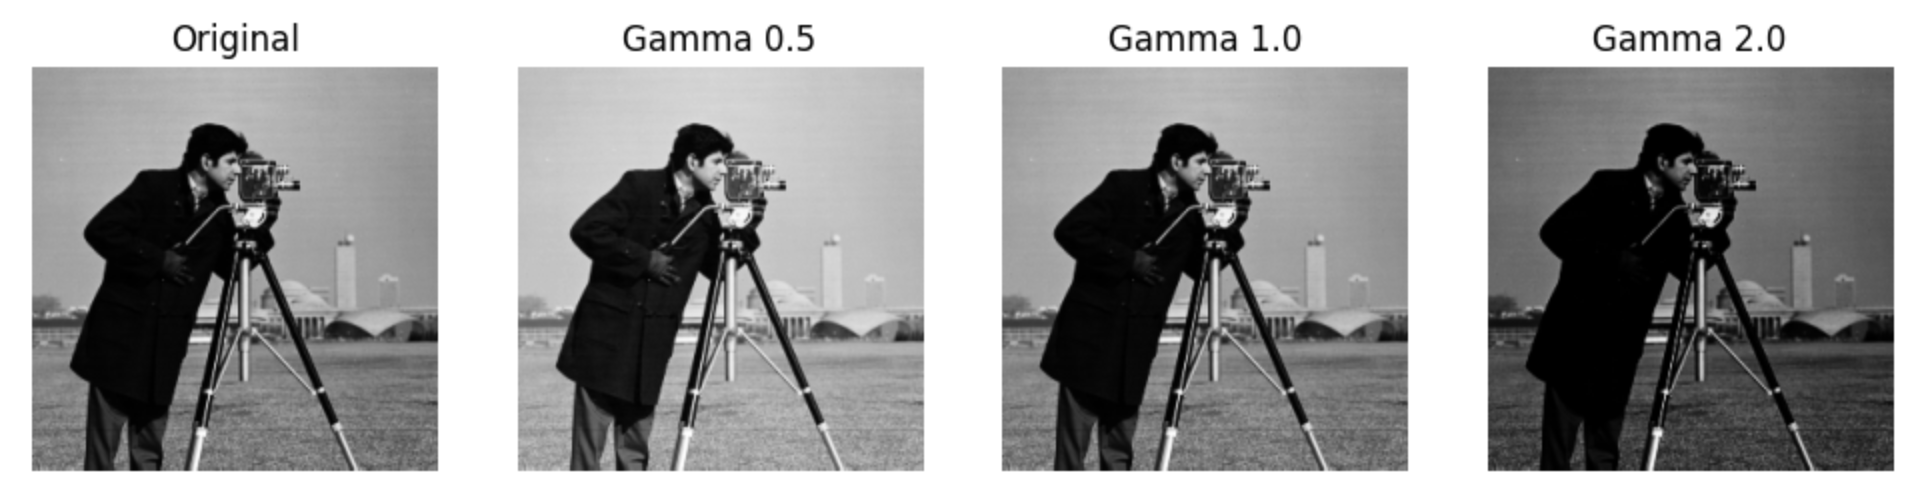
\includegraphics[width=0.7\columnwidth, keepaspectratio]{pics/a2-1.1}
\caption[]{Pixel-wise contrast enhancement on a gray scale picture}
\label{fig:1.1}
\end{figure}

\subsection{Color Image - RGB correction}

 See figure~\ref{fig:1.2} and Listing 2.

\begin{lstlisting} [caption={Gamma-RGB},captionpos=b]
def gamma_correct_rgb(image, gamma):
    corrected = np.zeros_like(image, dtype=np.uint8)
    for c in range(3): 
        corrected[..., c] = gamma_transform(image[..., c], gamma)
    return corrected
\end{lstlisting}
\begin{figure}[ht]
\centering
    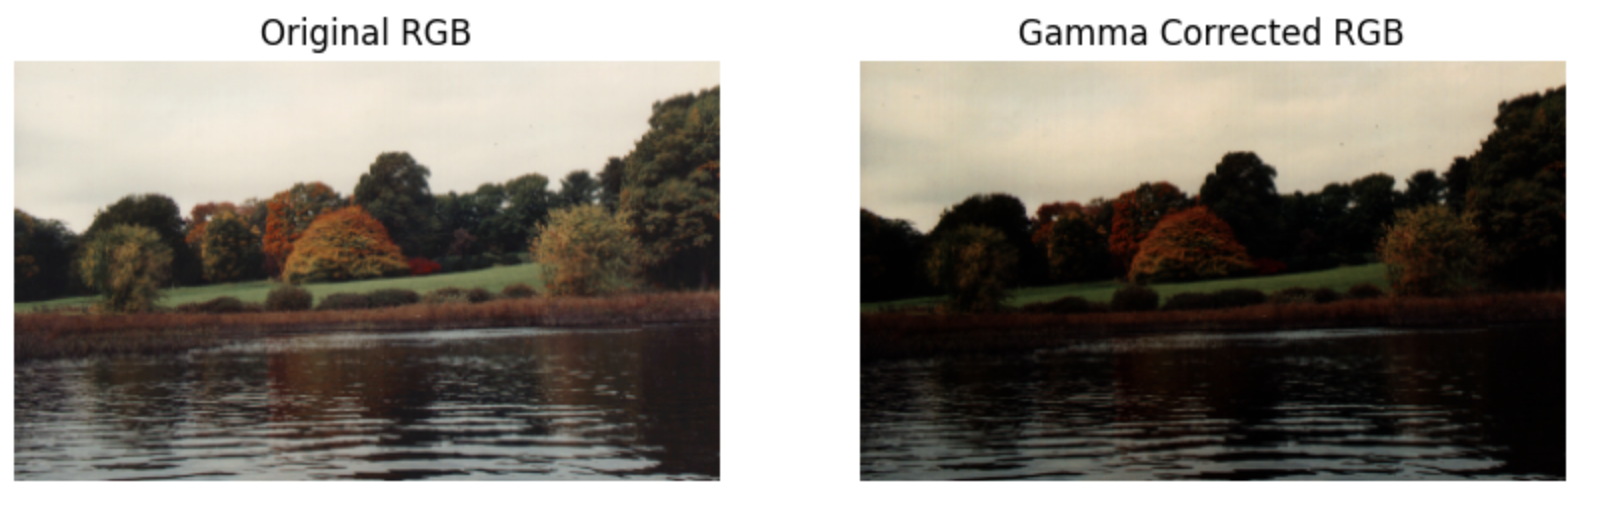
\includegraphics[width=0.7\columnwidth, keepaspectratio]{pics/a2-1.2}
\caption[]{Pixel-wise contrast enhancement on a gray scale picture}
\label{fig:1.2}
\end{figure}

\subsection{Color Image - HSV color representation}

\begin{lstlisting}[caption={Gamma-HSV},captionpos=b]
def gamma_correct_hsv(image, gamma):
    hsv_image = color.rgb2hsv(image)
    hsv_image[..., 2] = 
      gamma_transform(
      	(hsv_image[..., 2] * 255).astype(np.uint8), gamma) / 255.0
    return (color.hsv2rgb(hsv_image) * 255).astype(np.uint8)
\end{lstlisting}

 See figure~\ref{fig:1.3} and Listing 3.
 The result of the RGB Correction is a little more brighter on the bright part, and thus look less natural. This may because the RGB Correction alters all channels independently, and the colors may be distorted. The HSV Correction modifies only the brightness while preserving colors, so it looks better.

\begin{figure}[ht]
\centering
    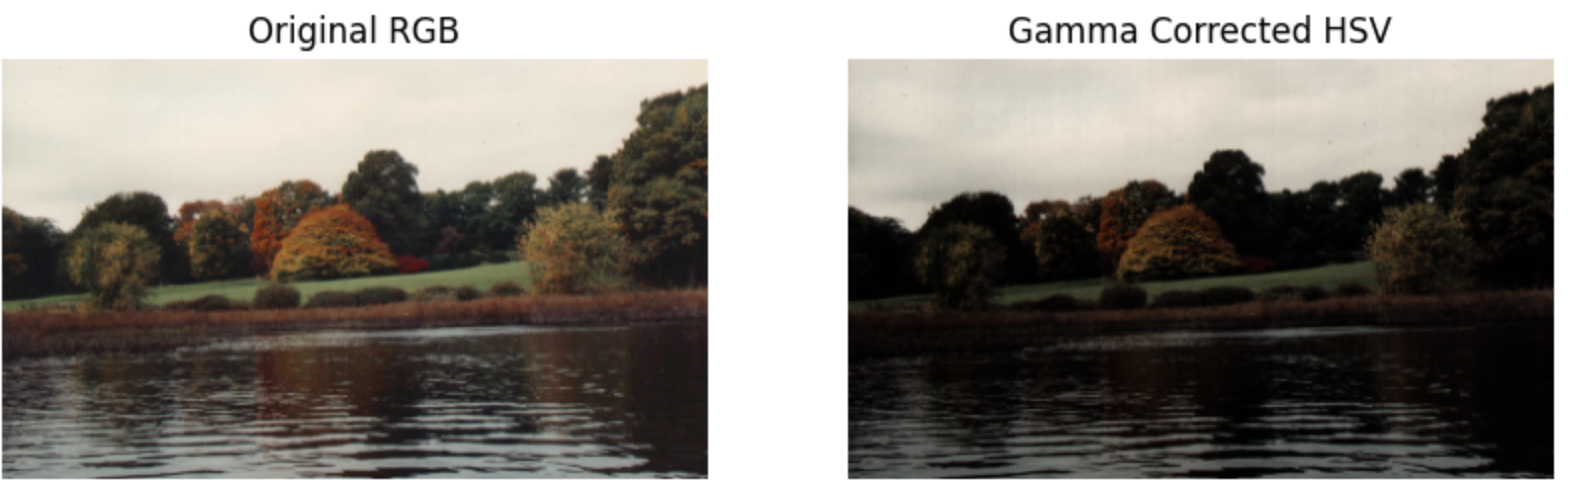
\includegraphics[width=0.7\columnwidth, keepaspectratio]{pics/a2-1.3}
\caption[]{Pixel-wise contrast enhancement on a gray scale picture}
\label{fig:1.3}
\end{figure}

\section{Reverb convolution}
%wanjing
\subsection{Plot laugh2.wav}
See figure ~\ref{fig:2.1}. The orange curve represents right sound track, and the blue curve represents the left sound track. The height of the curve represents the amplitude of this audio channel over time, with x-axis as time and y-axis as amplitude.
The sample rate represents how many samples per second are used to represent the sound.

\begin{figure}[ht]
\centering
    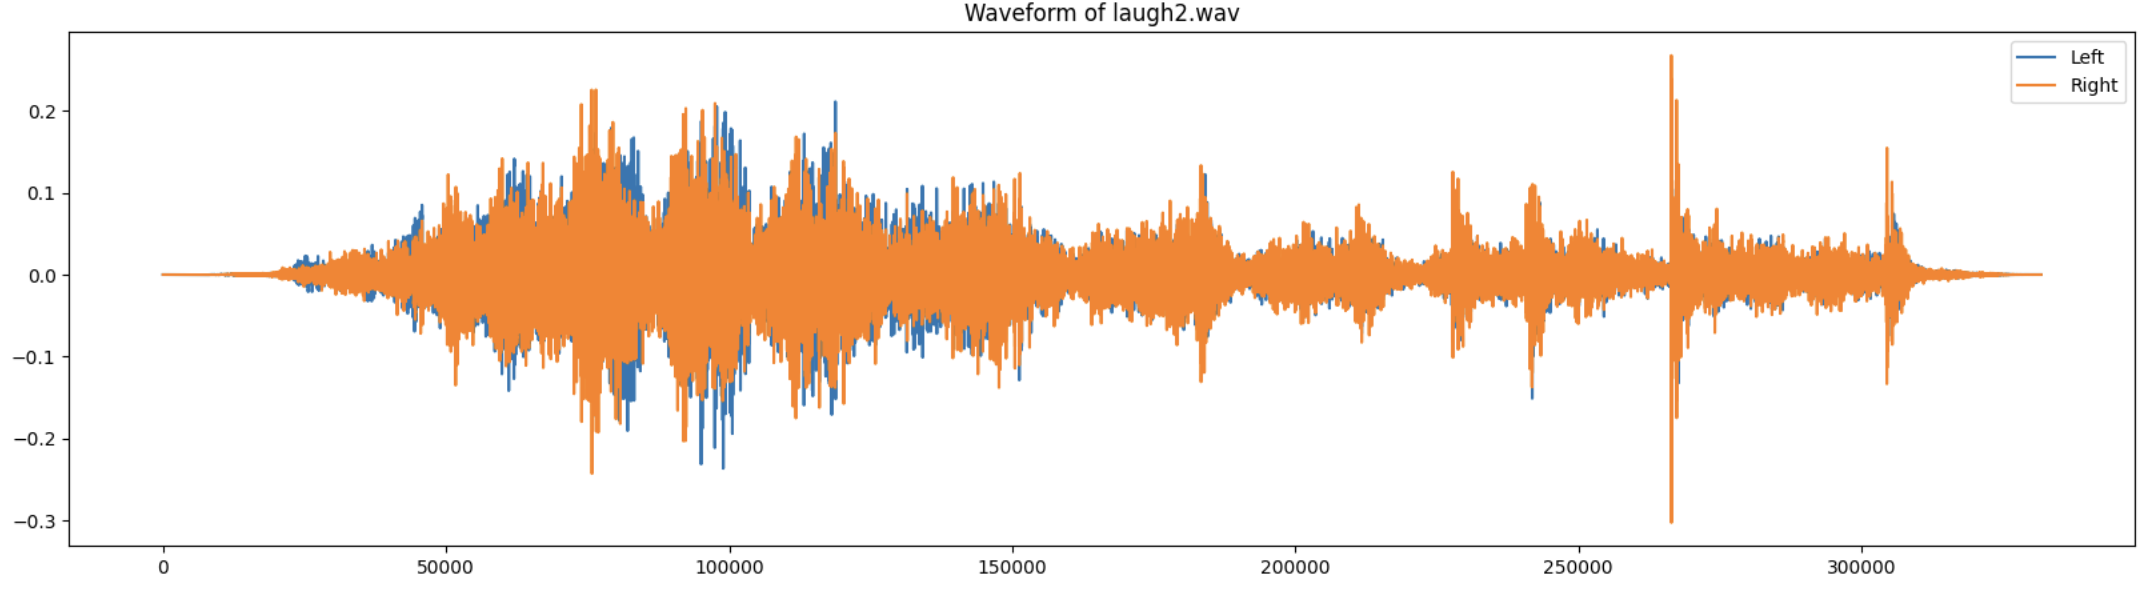
\includegraphics[width=0.7\columnwidth, keepaspectratio]{pics/a2-2.1}
\caption[]{Plot laugh2.wav}
\label{fig:2.1}
\end{figure}

\subsection{Reverb}

Reverb simulates sound reflections in space, making it feel more spacious and echoing.
With the convolution of Clap, the reverb mix the clap and the origin laughter, and it sounds like the laughter is mixed with claps in a hall. See ~\ref{fig:2.2.2} for Clap result, and the origin is in ~\ref{fig:2.2.1}.
With the convolution of Splash, the laughter sounds like coming from the outer space.  See ~\ref{fig:2.2.3}.
\begin{figure}[ht]
\centering
\subfigure[Original Signal]{
    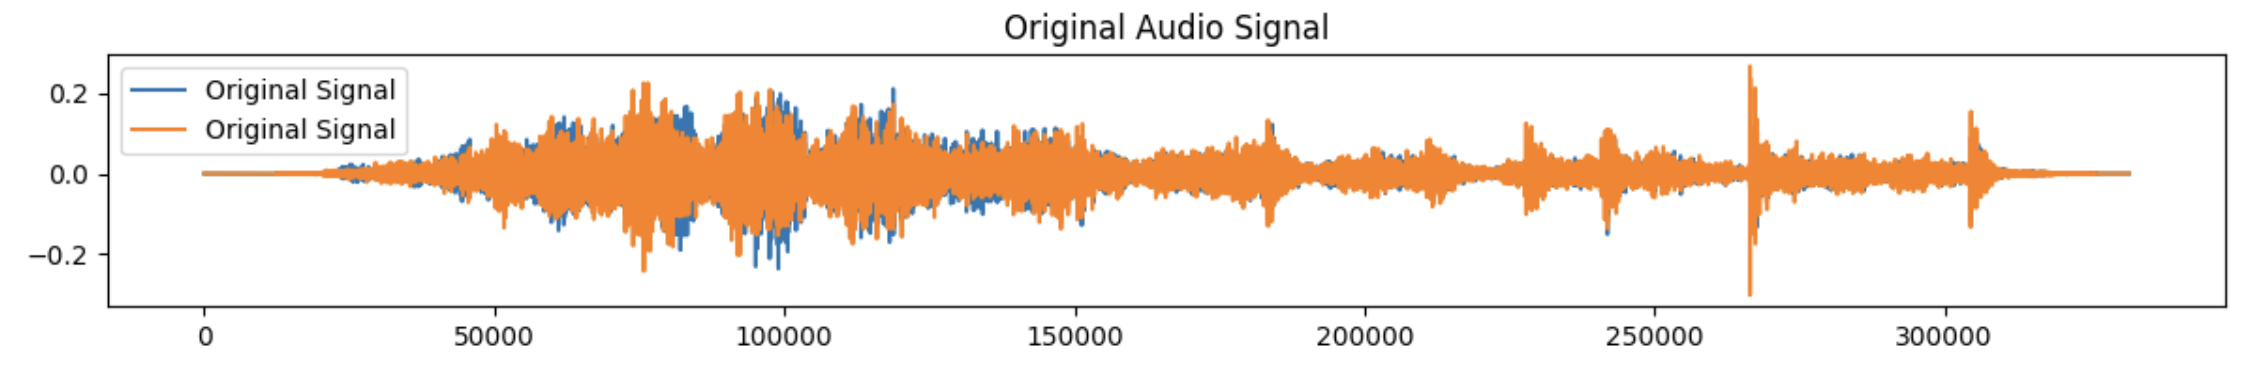
\includegraphics[width=0.7\columnwidth, keepaspectratio]{pics/a2-2.2-origin}
\label{fig:2.2.1}
}
\subfigure[Response Signal, Clap]{
    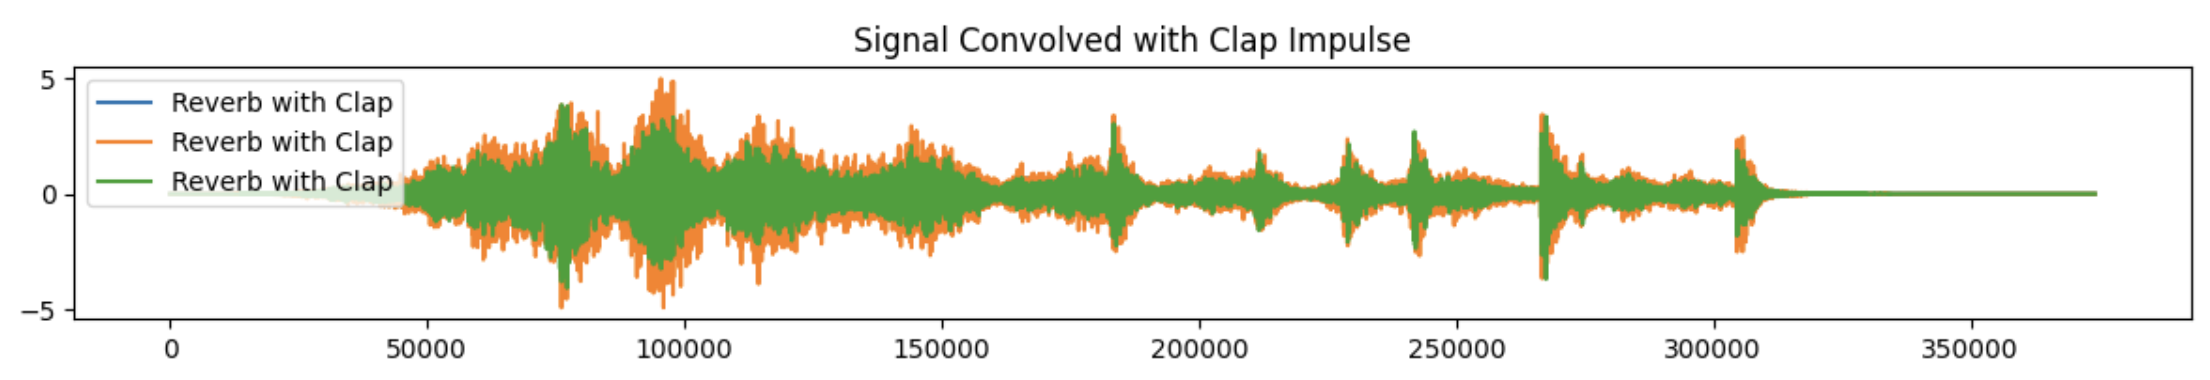
\includegraphics[width=0.7\columnwidth, keepaspectratio]{pics/a2-2.2-clap}
\label{fig:2.2.2}
}
\subfigure[Response Signal, Splash]{
    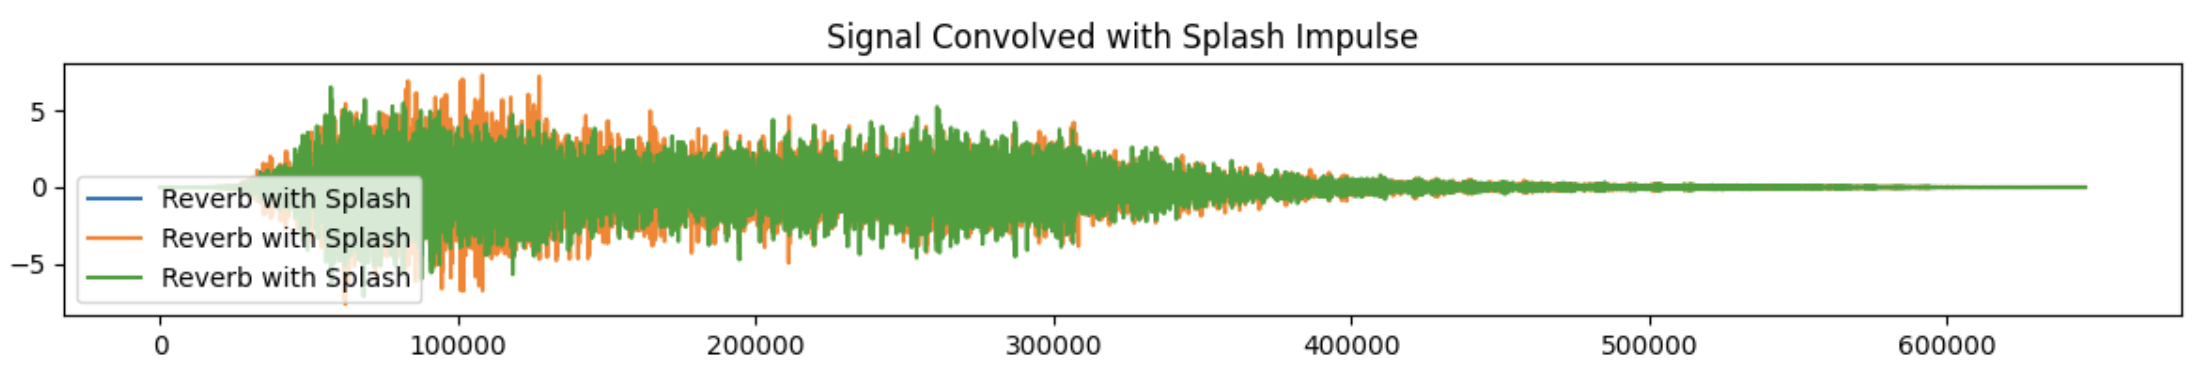
\includegraphics[width=0.7\columnwidth, keepaspectratio]{pics/a2-2.2-splash}
\label{fig:2.2.3}
}
\caption[]{Plot laugh2.wav}
\label{fig:2.2}
\end{figure}


\subsection{Longer explanation}

The convolution operation matches the two inputs and do calculation. The output size is $len(signal)+len(impulse)-1$. In our case, the convolution blends the original waveform with the impulse response and adds tail reflections.

\section{Image filtering and enhancement}
%zhigao

\subsection{}
Figure 6 shows the original image as well as the image with salt and pepper noise and gaussian noise added.
\begin{figure}[ht]
    \centering
        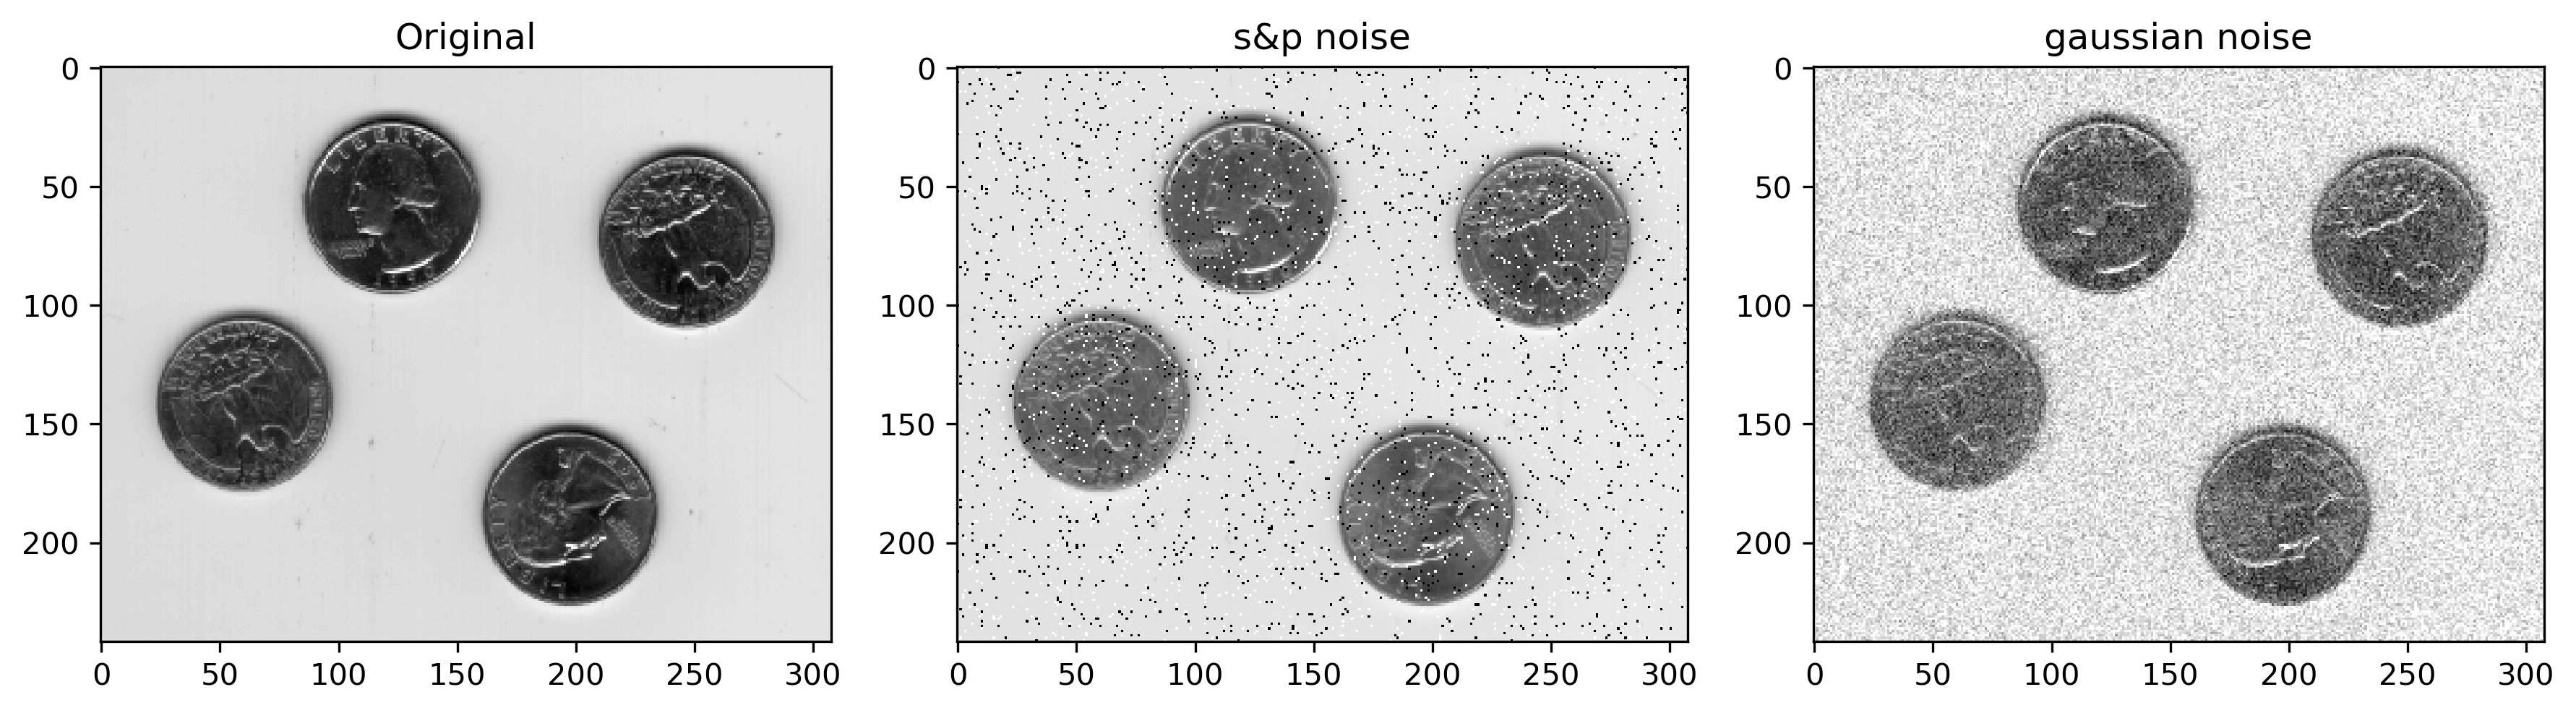
\includegraphics[width=1\columnwidth, keepaspectratio]{pics/a2-3.1-1}
    \caption[]{Original image and images with different types of noise}
    \label{fig:3.1}
    \end{figure}
   
    \begin{figure}[ht]
        \centering
            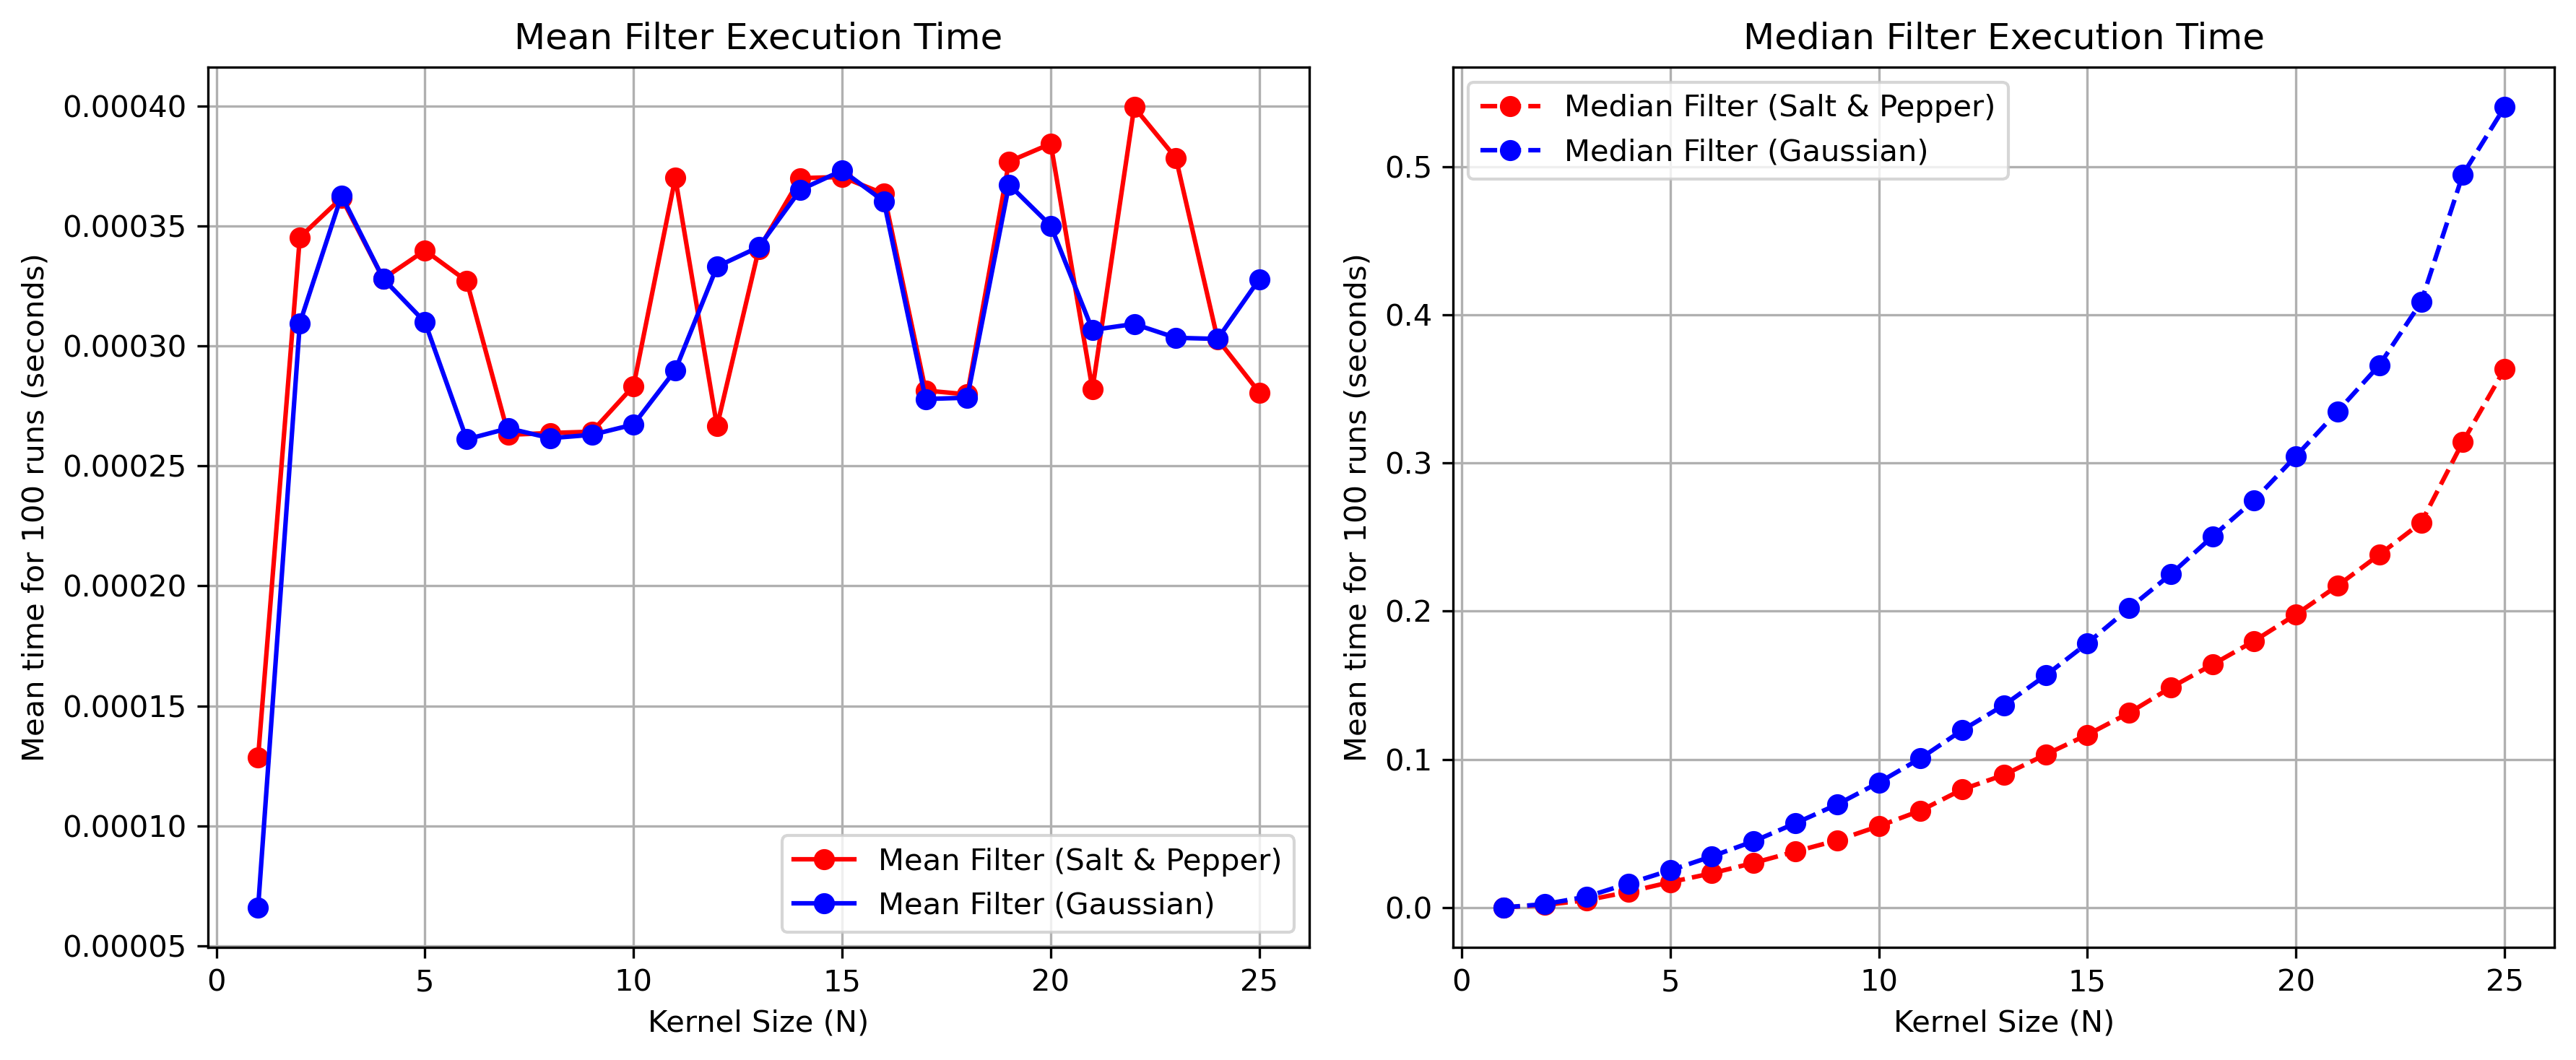
\includegraphics[width=1\columnwidth, keepaspectratio]{pics/a2-3.1-2}
        \caption[]{Different Average times obtained for N=1 to N=25 and each time for 100 executions}
        \label{fig:3.2}
        \end{figure}
        From figure 7, The computational time for Mean filter is low and varies less with kernel size, whereas the computational time for Median filter grows exponentially with kernel size and is particularly time-consuming for Gaussian noise. 
    \begin{figure}[ht]
        \centering
            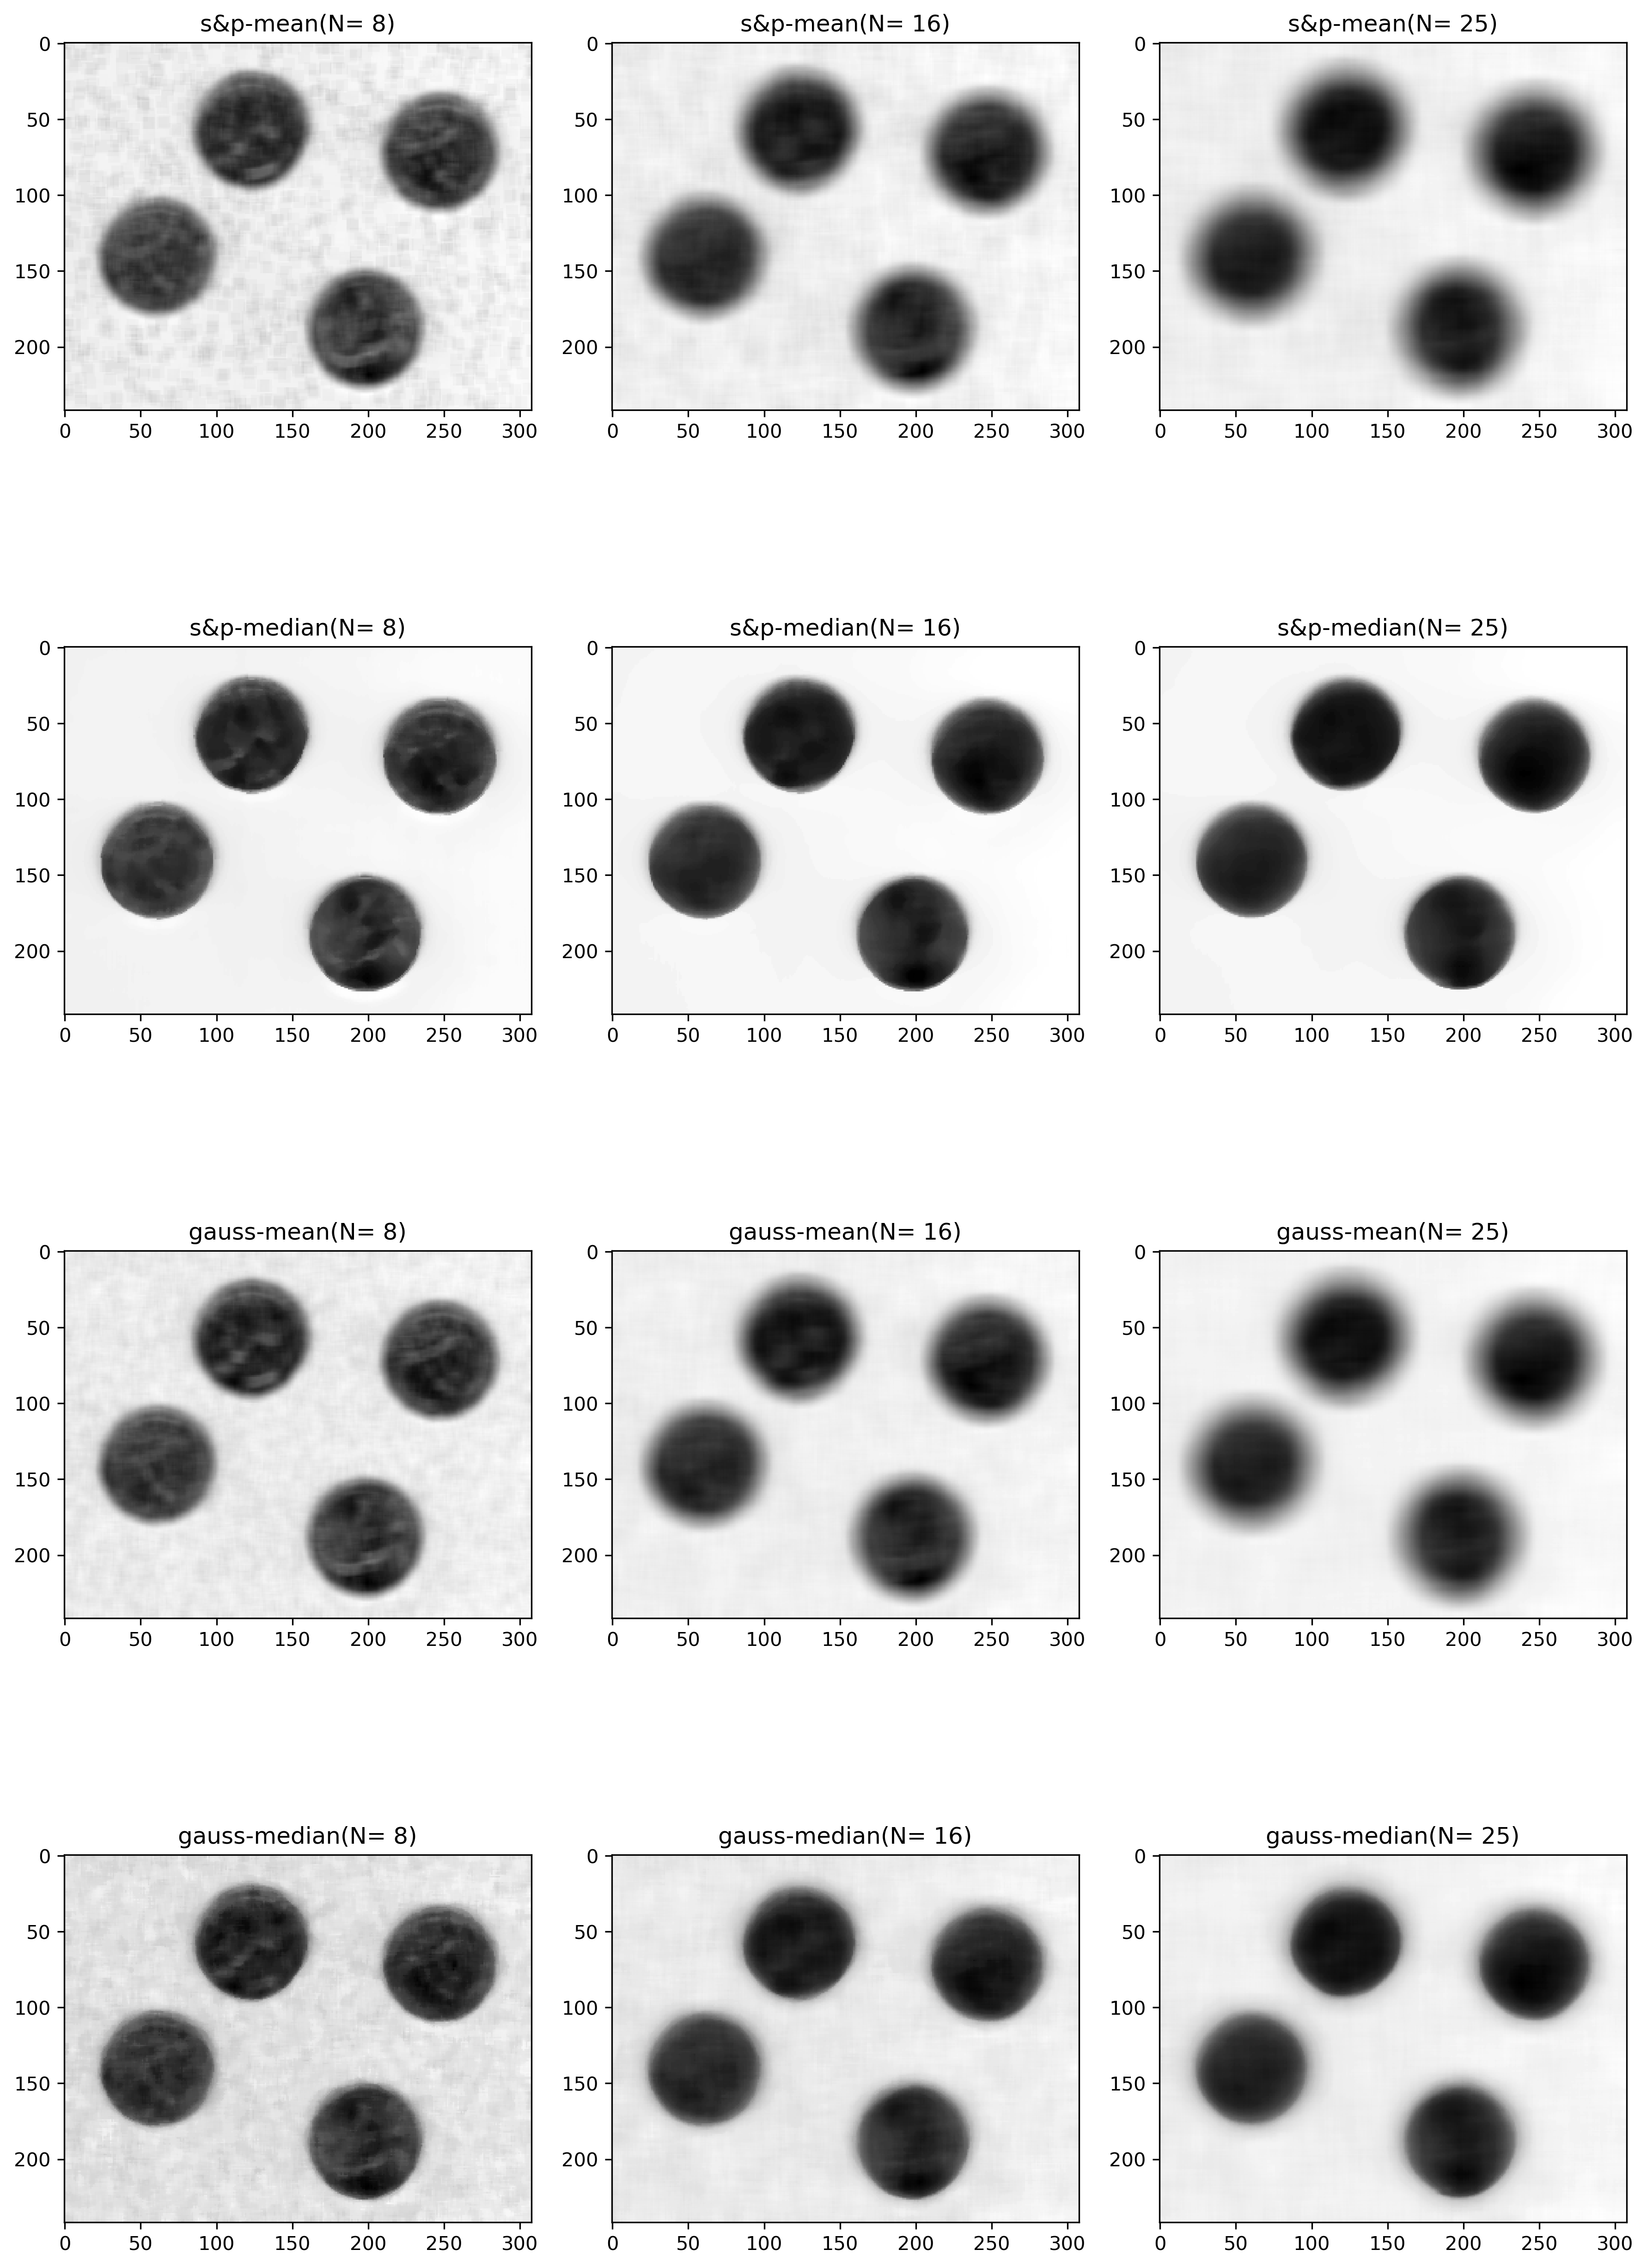
\includegraphics[width=0.5\columnwidth, keepaspectratio]{pics/a2-3.1-3}
        \caption[]{Visual effect of image with different types of noise by increasing the kernel size N }
        \label{fig:3.3}
    \end{figure}
    
    
    For figure 8, As the kernel size N increases, the filtering effect increases and the image becomes blurrier. The effect of smoothing the noise by Mean filter is obvious, but it will lead to blurring of edges, especially when 
    N = 25, the details are lost severely. The Median filter removes salt and pepper noise better and retains image edge detail better. Even though N increases, it still retains more detail than the mean filter.
    \subsection{}  
    \begin{figure}[ht]
        \centering
            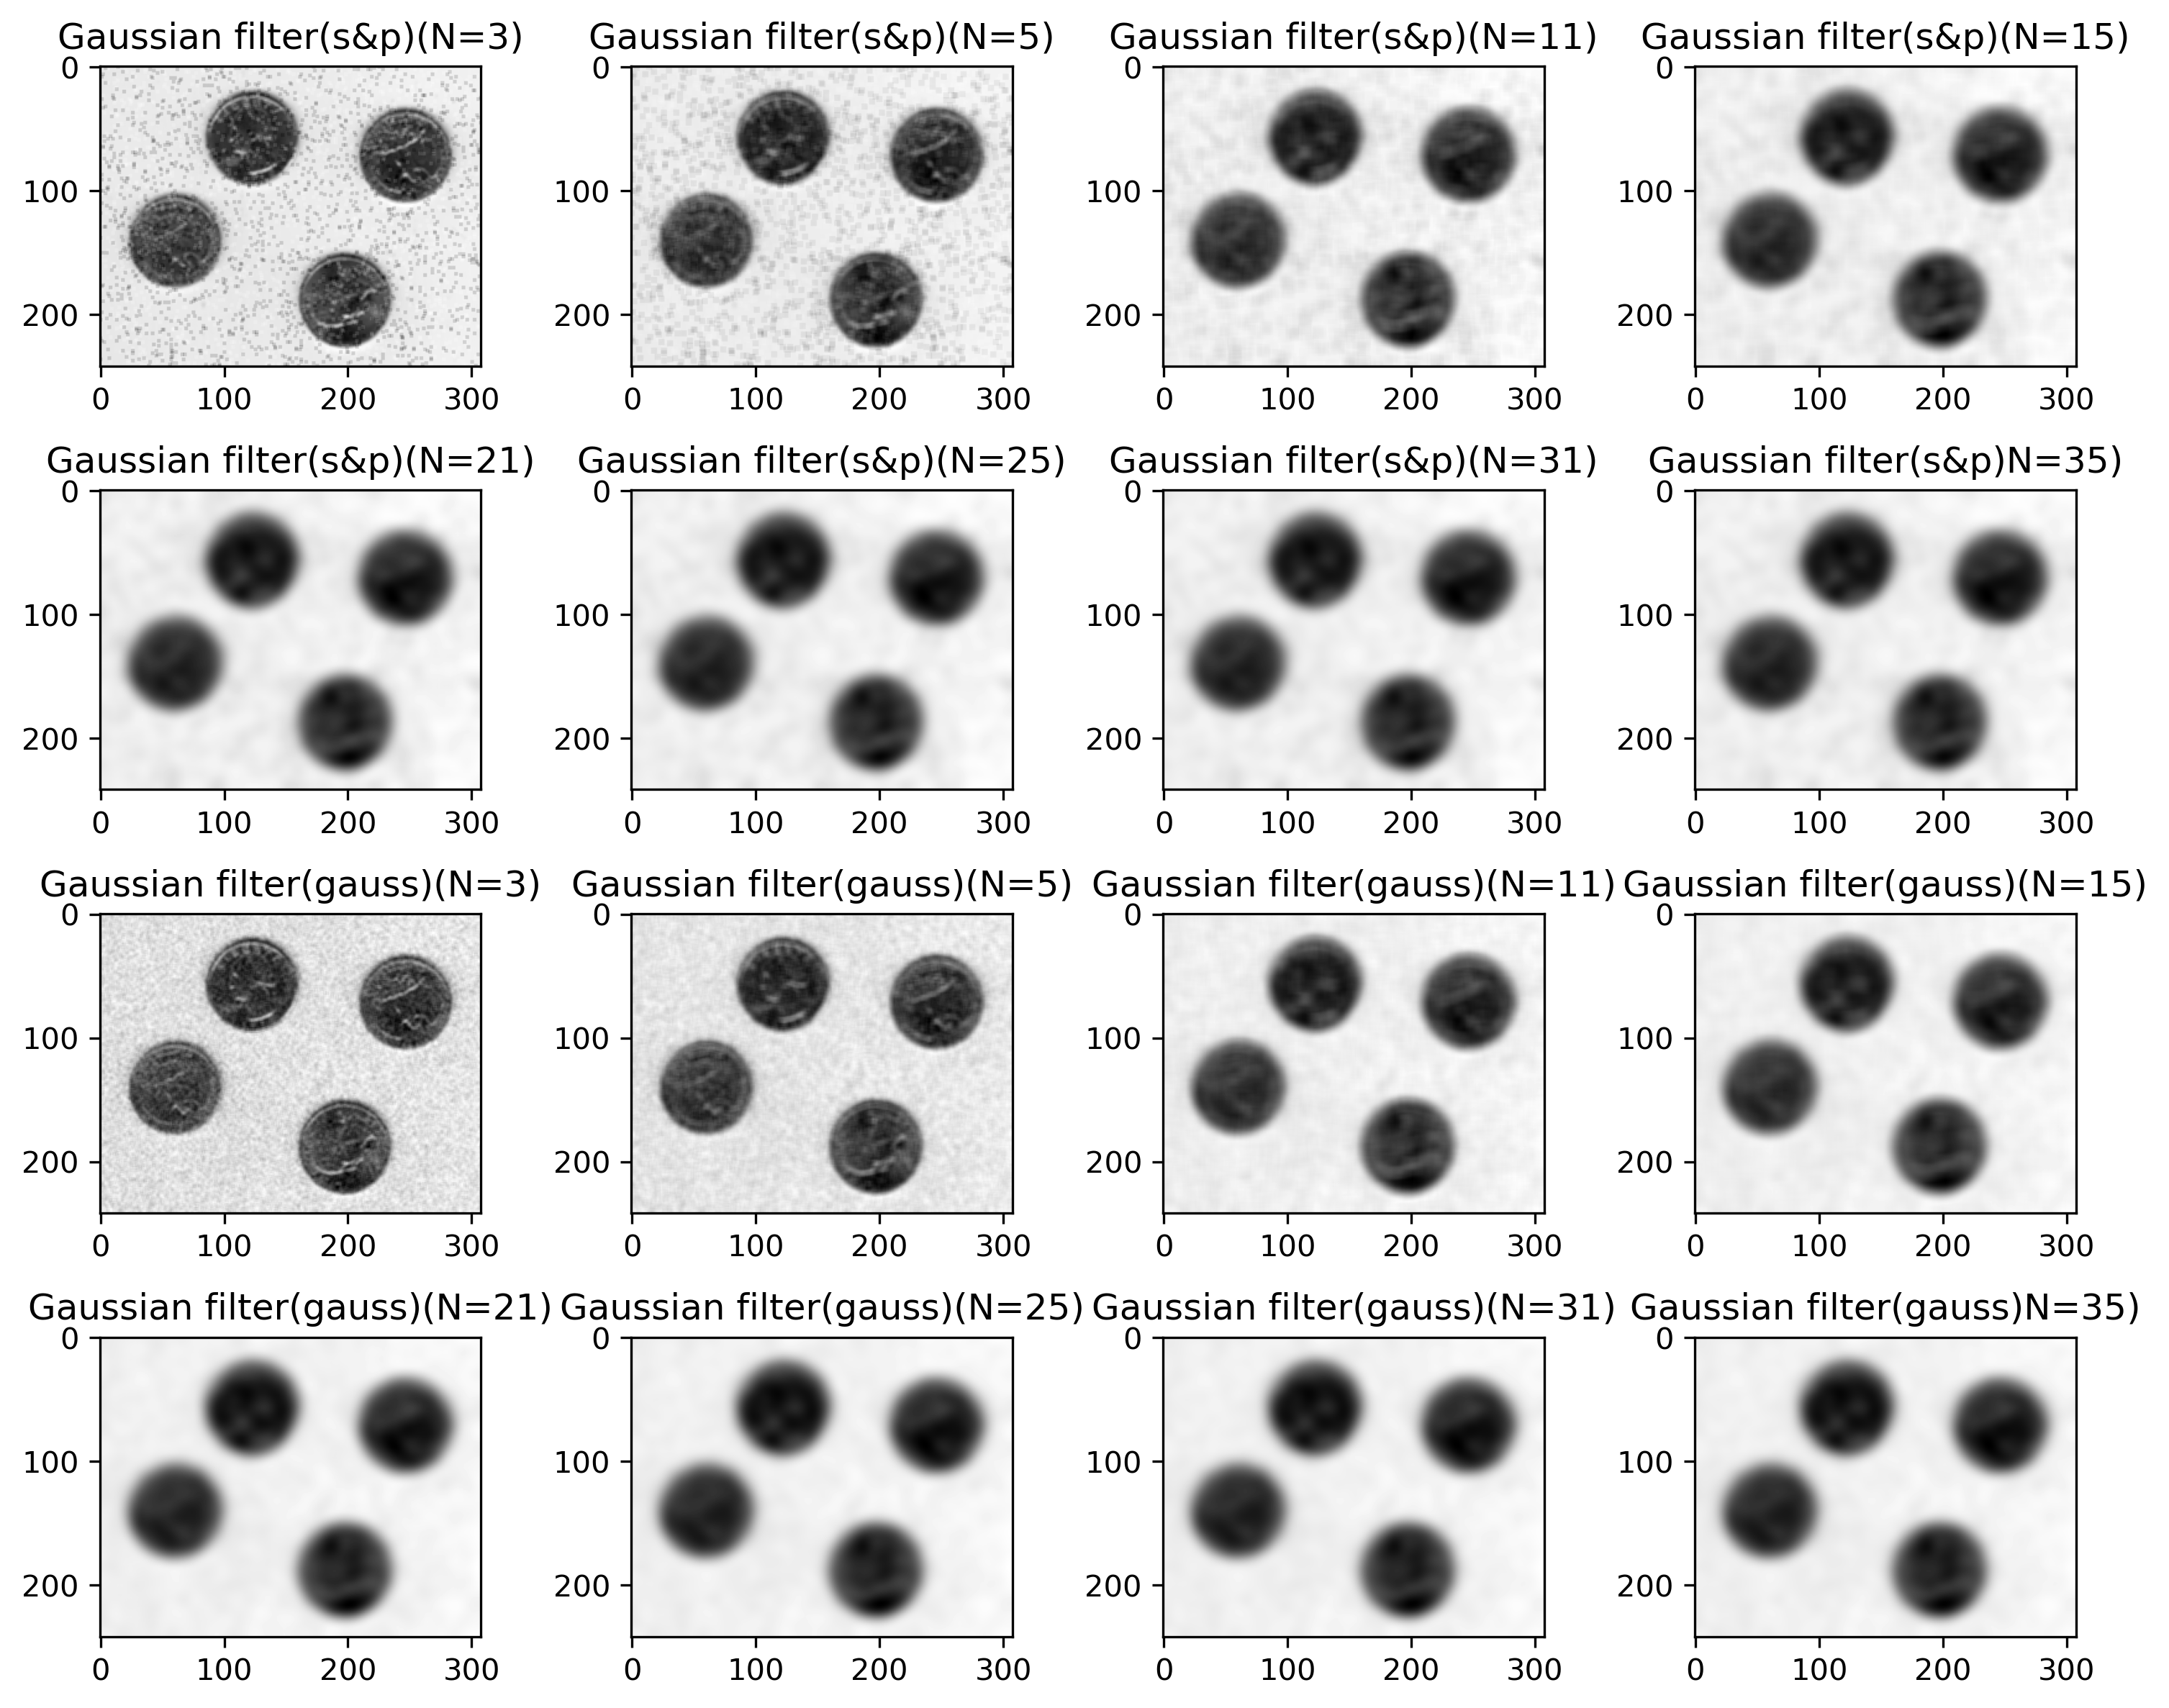
\includegraphics[width=0.7\columnwidth, keepaspectratio]{pics/a2-3.2}
        \caption[]{The effect of gaussian filter for different kernel size N(Sp and Gaussian noise)}
        \label{fig:3.4}
    \end{figure}
    From Figure 9, I think that when N exceeds 21, the visual effect of the image no longer changes significantly. I think the reason for this is that when N is large enough, the Gaussian kernel acts close to the entire image. At this point the image can also be considered as a large uniform blur. So even if N is increased, there is no significant change in the image.


    \subsection{}
    \begin{figure}[ht]
        \centering
            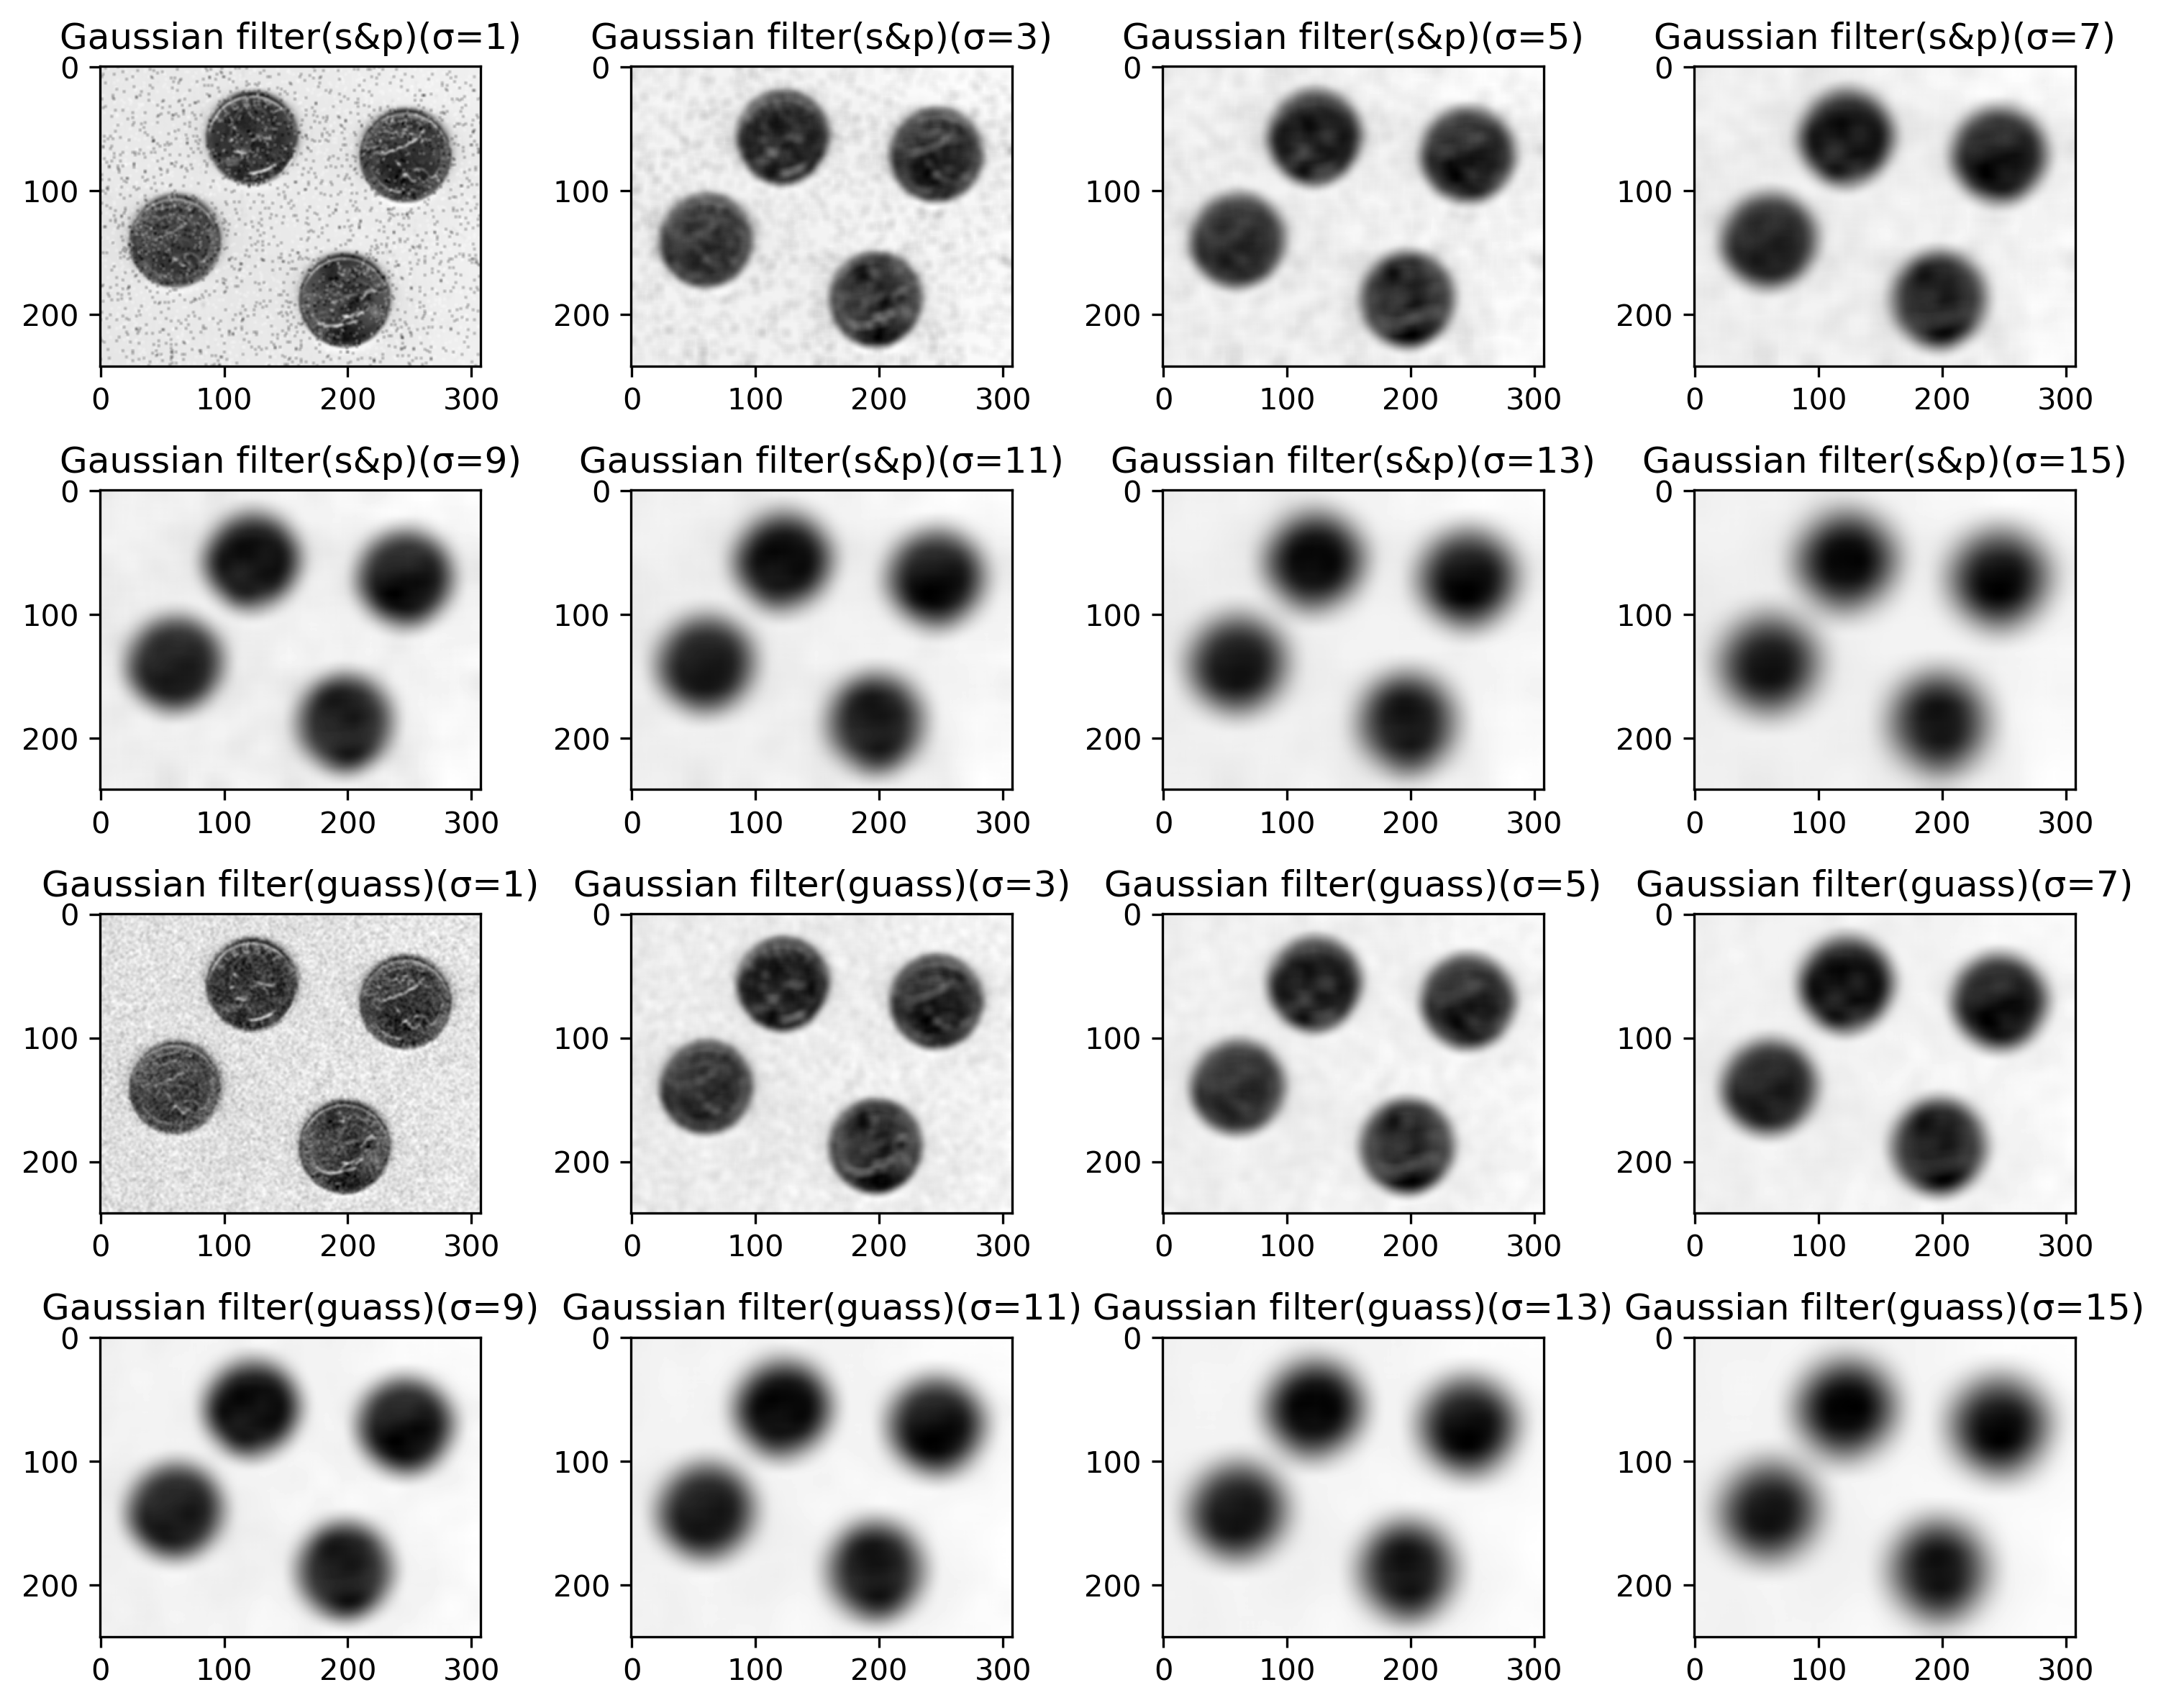
\includegraphics[width=0.7\columnwidth, keepaspectratio]{pics/a2-3.3}
        \caption[]{The effect of gaussian filter for different sigma(Sp and Gaussian noise)}
        \label{fig:3.5}
    \end{figure}
    From figure 10, I found that Gaussian filter is suitable for removing Gaussian noise, not for salt and Pepper noise. Too little $\sigma$ is not enough for denoising and too much $\sigma$ causes blurring, That is, the image loses a lot of sharpness. I think $\sigma$ = 7 - 9 is recommended as the best balance point, But it is also depends on the level of noise.
\section{Histogram-based processing}
\subsection{}
\begin{lstlisting}[caption={CDF Calculation},captionpos=b]
def compute_cdf(image):
    hist, _ = np.histogram(image.flatten(), bins=256, range=[0, 256])
    cdf = np.cumsum(hist).astype(np.float32)
    cdf /= cdf[-1]  # Normalize to [0,1]
    return hist, cdf
\end{lstlisting}

\begin{figure}[ht]
        \centering
            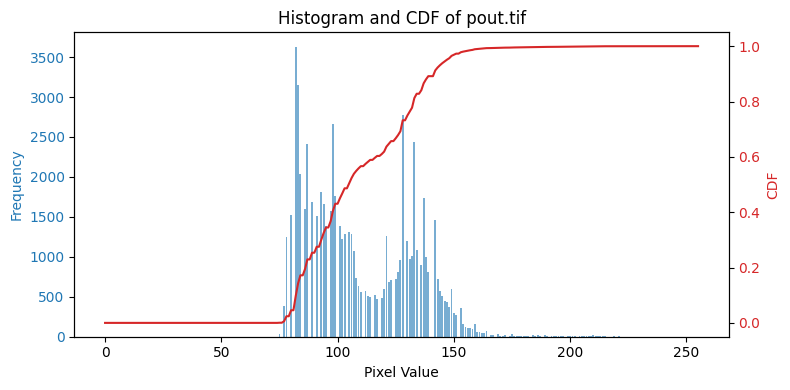
\includegraphics[width=0.7\columnwidth, keepaspectratio]{pics/a2-4.1}
        \caption[]{Computing the CDF for pout.tif}
    \label{fig:4.1}
    \end{figure}

Figure \ref{fig:4.1} shows the result of computing the CDF for the image pout.tif using your function.

The areas where CDF increases rapidly (about 80-150) indicate that the pixel values in these areas appear frequently, which means that most of the pixels in the image are in this grayscale range. Corresponding to the original image, it may be the background or a large area of clothing.
The areas where CDF is flat represent
the low grayscale part (0-50) and the high grayscale part (above 200). This means that the frequency of occurrence of these pixel values is very low, and there are almost no particularly dark or bright areas in the image. This reflects that the contrast of the original image is low, and the pixel values are concentrated in the medium grayscale area, which makes the image look dark and not vivid enough.

\subsection{}
\begin{lstlisting}[caption={Apply CDF Transformation to Image},captionpos=b]
def apply_cdf(image, cdf):
    cdf_mapped = np.round(cdf * 255).astype(np.uint8)
    equalized_image = cdf_mapped[image]
    return equalized_image
\end{lstlisting}

Figure \ref{fig:4.2} shows the result of applying this function to the pout.tif image.
\begin{figure}[ht]
        \centering
            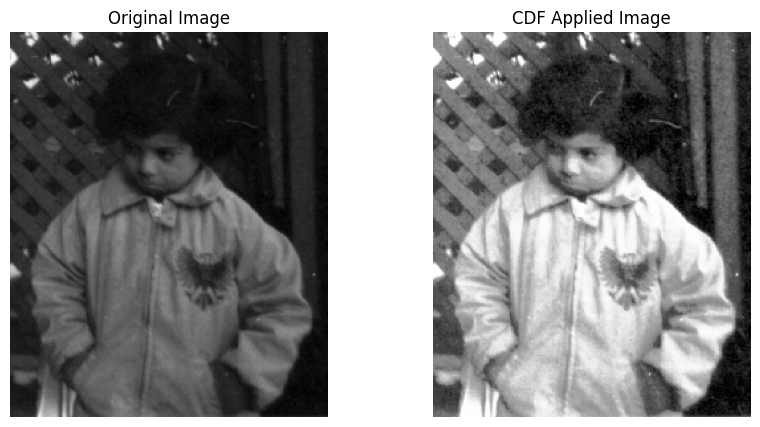
\includegraphics[width=0.7\columnwidth, keepaspectratio]{pics/a2-4.2}
        \caption[]{Apply CDF to pout.tif}
    \label{fig:4.2}
    \end{figure}

\subsection{}

Answer to the question:
In some grayscale value intervals, pixel values may not appear, resulting in a flat area in the CDF. In these areas, the derivative of the CDF is 0, and the reverse mapping cannot be uniquely determined. At the same time, the pixel value is discrete (0-255), while the CDF is a continuous cumulative curve in mathematics, which may result in no unique solution for the mapped pixel value.

\begin{lstlisting}[caption={Compute Inverse CDF},captionpos=b]
def compute_inverse_cdf(cdf):
    intensity_levels = np.linspace(0, 255, 256)
    inverse_cdf = np.interp(np.linspace(0, 1, 256), cdf, intensity_levels)
    return np.clip(np.round(inverse_cdf), 0, 255).astype(np.uint8)

\end{lstlisting}

\subsection{}

\begin{lstlisting}[caption={Perform Histogram Matching between Two Images},captionpos=b]
def ensure_numpy_array(cdf):
# Ensure that the given CDF is a NumPy array.
    if isinstance(cdf, tuple):
        cdf = np.array(cdf[0])
    else:
        cdf = np.array(cdf)
    return cdf

def histogram_matching(source_image, target_image):

    _, cdf_source = compute_cdf(source_image)
    _, cdf_target = compute_cdf(target_image)

    inverse_cdf_target = compute_inverse_cdf(cdf_target)

    # Normalize source image intensity to CDF space
    source_cdf_values = cdf_source[source_image]

    # Map source CDF values to target intensity values
    matched_image = np.interp(source_cdf_values, np.linspace(0, 1, 256), inverse_cdf_target)

    # Convert to uint8 and clip values
    matched_image = np.clip(matched_image, 0, 255).astype(np.uint8)

    return matched_image
\end{lstlisting}

Figure \ref{fig:4.4-1} shows the results of the histogram matching between two images.

\begin{figure}[ht]
        \centering
            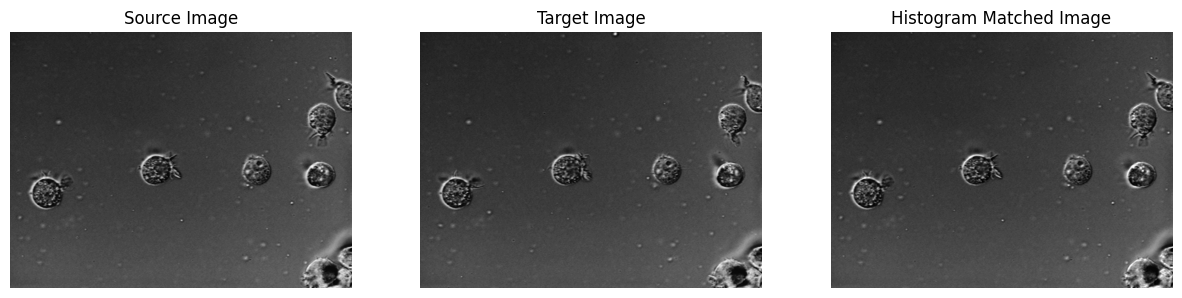
\includegraphics[width=0.7\columnwidth, keepaspectratio]{pics/a2-4.4-1.png}
        \caption[]{Perform Histogram Matching between Two Images}
    \label{fig:4.4-1}
    \end{figure}

Figure \ref{fig:4.4-2} shows the cumulative distribution function (CDF) of the original image, the target image, and the image after histogram matching:
The CDF of the matched image is very close to the CDF of the target image, indicating that the histogram matching successfully adjusted the pixel distribution.
The CDF remains monotonically increasing, ensuring that the pixel value mapping is reasonable and there are no obvious artifacts.
Overall, the histogram matching method effectively adjusts the original image to make its pixel distribution closer to the target image.
\begin{figure}[ht]
        \centering
            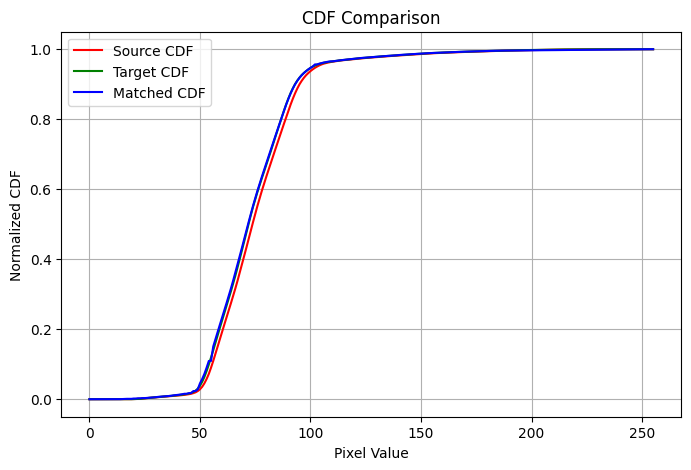
\includegraphics[width=0.7\columnwidth, keepaspectratio]{pics/a2-4.4-2.png}
        \caption[]{Cumulative Histograms Comparison}
    \label{fig:4.4-2}
    \end{figure}

\end{document}



